\documentclass[]{myclass}
\usepackage[cp1250]{inputenc}
\usepackage[OT4]{fontenc}

\usepackage[table,xcdraw]{xcolor}
\usepackage{multirow}
\usepackage{subfig}
\usepackage{float}
\usepackage{amsfonts}
\usepackage{pdfpages}
\usepackage{listings}
\usepackage[english]{babel}
\usepackage{titling}
\usepackage{tocbibind}
\usepackage[all]{nowidow}
\usepackage{comment}
\usepackage{caption}
\usepackage{indentfirst}
\usepackage{amsmath} %subeq
\usepackage{mathtools} %split eq

\definecolor{mygreen}{rgb}{0,0.6,0}
\lstset {
basicstyle=\small,
breaklines=true,
commentstyle=\color{mygreen},
keywordstyle=\color{blue},
language=C,
linewidth=\textwidth
}
\linespread{1}

\author{Marcin Aftowicz}
\title{Hardware Test and fault diagnosis based on extended FEC functions  in wireless communication systems}
\mysupervisor{Prof. Dr.-Ing. H. T. Vierhaus \and Ing. Petr Pfeifer, MSc, MBA, Ph.D.}
\myyear{2018}
\usepackage{hyperref}
\hypersetup{
    linkcolor={blue!70!black},
    citecolor={blue!70!black},
    urlcolor={blue!70!black}
}
\begin{document}
\selectlanguage{english}
\bibliographystyle{plplain}

% Front matter **************************************
\frontmatter
\pagestyle{empty}%
\maketitle  \cleardoublepage

\pagenumbering{Roman}
\phantomsection
\addcontentsline{toc}{chapter}{Statutory declaration}

{\noindent}STATUTORY DECLARATION\\

I declare that I have authored this thesis independently, that I have not used other than the declared 
sources  /  resources,  and  that  I  have  explicitly  marked  all  material  which  has  been  quoted  either  
literally or by content from the used sources. \\
\par\vspace{15mm}\par

Marcin Aftowicz \hfill Date \hspace{2cm}

   \cleardoublepage

\pagestyle{ppfcmthesis}
\phantomsection
\addcontentsline{toc}{chapter}{Abstract}
\begin{abstract}
Wireless communication is more and more commonly used in highly unfavorable environments. Nowadays it's not only cellular communication, but also communication within cities, industrial production facilities and other short distance, real-time applications. Such systems have significant demand on safety whilst being vastly exposed not only to signal interferences, multi-path signal propagation and fading effects, but also to transient and permanent faults in hardware. While communication errors are covered by increasingly effective error correcting codes, the permanent faults in hardware still pose a threat to dependability. Since the communication systems consist of digital, analog and mixed-signal circuitry, the diagnostic test to uncover permanent faults happens in every module separately. The test extensions have to be built in during the development process, which is difficult in systems with no access to the internal structure of some IPs, e.g. due to patent protection. The following thesis describes the implementation of a diagnostic test, while treating the communication system as a whole and using the forward error correction units for error position determination.
\vfill


 \noindent Marcin Aftowicz m.j.aftowicz@gmail.com \newline


\end{abstract}    \cleardoublepage

\listoffigures  \cleardoublepage
\listoftables   \cleardoublepage

\tableofcontents \cleardoublepage

% Main matter **************************************
\mainmatter
 
%Define necessary functions for diagnostic tests	   
%Define encoder/decoder extensions	   
%Implement extensions on FPGAs	   
%Develop diagnostic test interface software to control / set optional parameters and record results	   
%Implement into FPGA an experimental set-up	   
%Conduct measurements on examples

%das Block-Diagramm zu ParSec zeigen
%zeigen wie der Baseband-Prozessor aufgebaut ist (digital-analog), so dass ein direkter interner Test mit bekannten "digitalen" Verfahren schwierig ist.
%vorstellen, dass man bei einem System wie in ParSec ohne FEC nicht auskommt.
%Zeigen, dass FEC-Komponenten partiell eigene Fehler korrigieren.
%zeigen (Petr!) wie man bei den FEC-Komponenten Selbsttest-Funktionen einbauen kann.

%=============================================================
\input{"1_introduction.tex"}
%=============================================================
\input{"2_dependability"}
%=============================================================
\input{"3_test.tex"}
%=============================================================
\input{"4_experiment.tex"}
%=============================================================
\input{"5_test_bench.tex"}

% All appendices and extra material, if you have any.
\cleardoublepage
\appendix%

%\chapter{Rysunki techniczne}
\begin{figure} [h]
\centering
%%----start of first subfigure----
	\subfloat[G�rna warstwa p�ytki]{\label{fig:subfig:front} 
	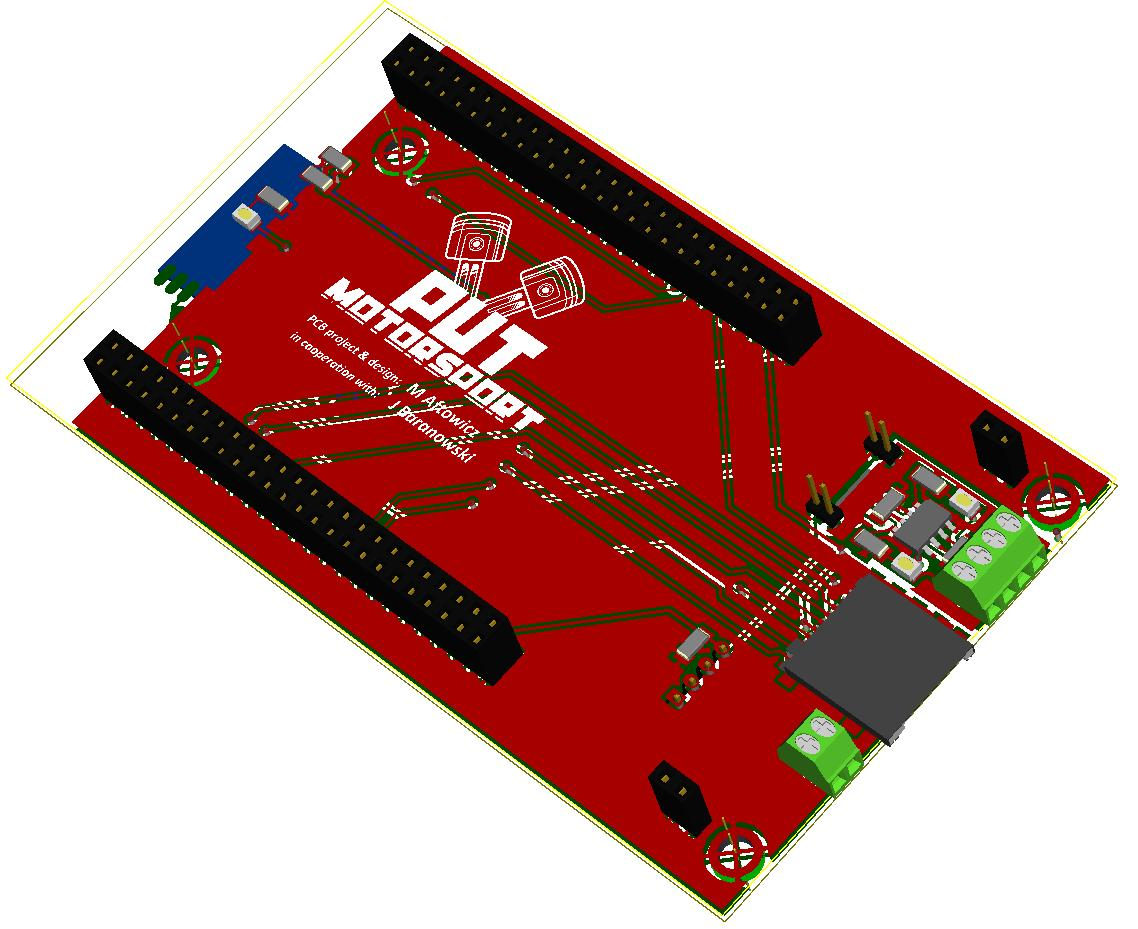
\includegraphics[height=0.3\textheight]{figures/Board_PCB_front.JPG}}
	\hfill
%%----start of second subfigure----
	\subfloat[Dolna warstwa p�ytki]{\label{fig:subfig:back}
	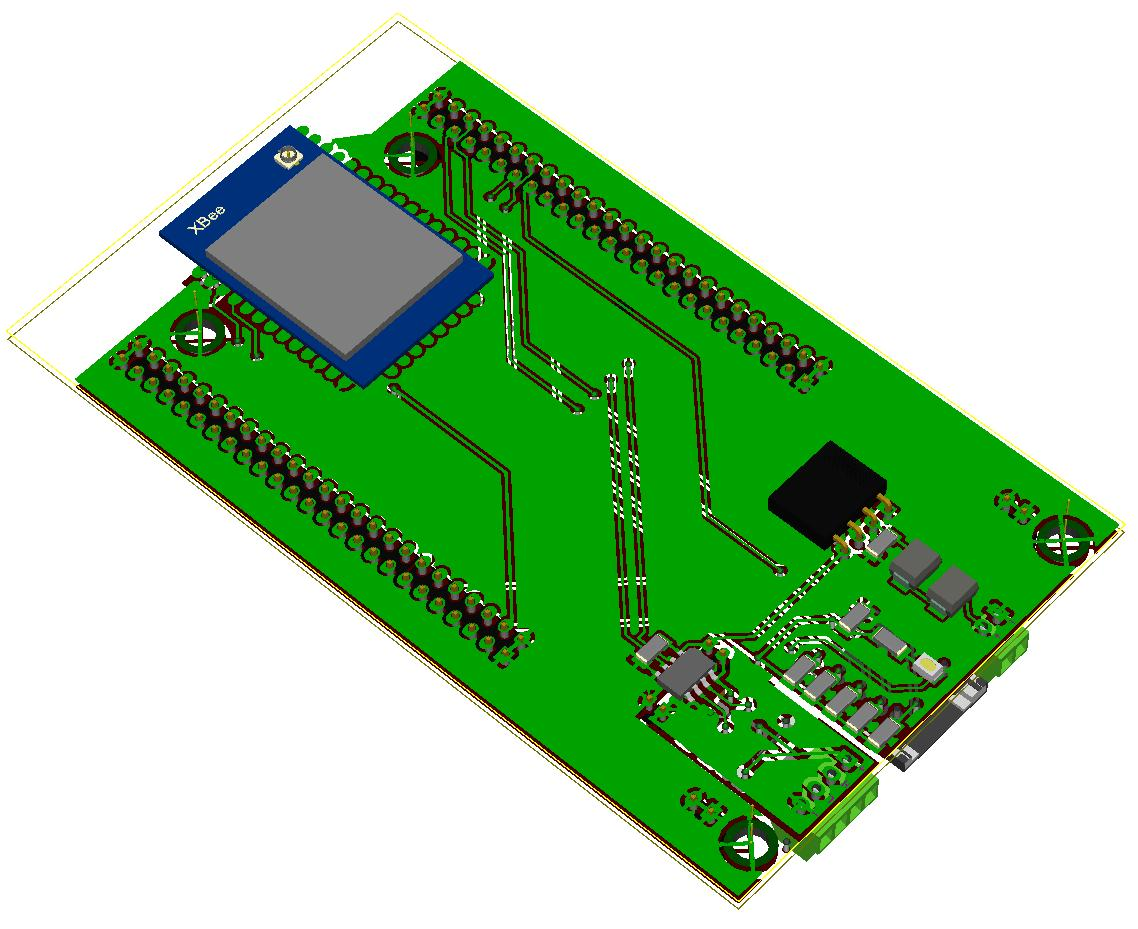
\includegraphics[height=0.3\textheight]{figures/Board_PCB_back.JPG}}
	\caption{Model 3D nak�adki na Discovery}
	\label{fig:3D} %% label for entire figure
\end{figure}

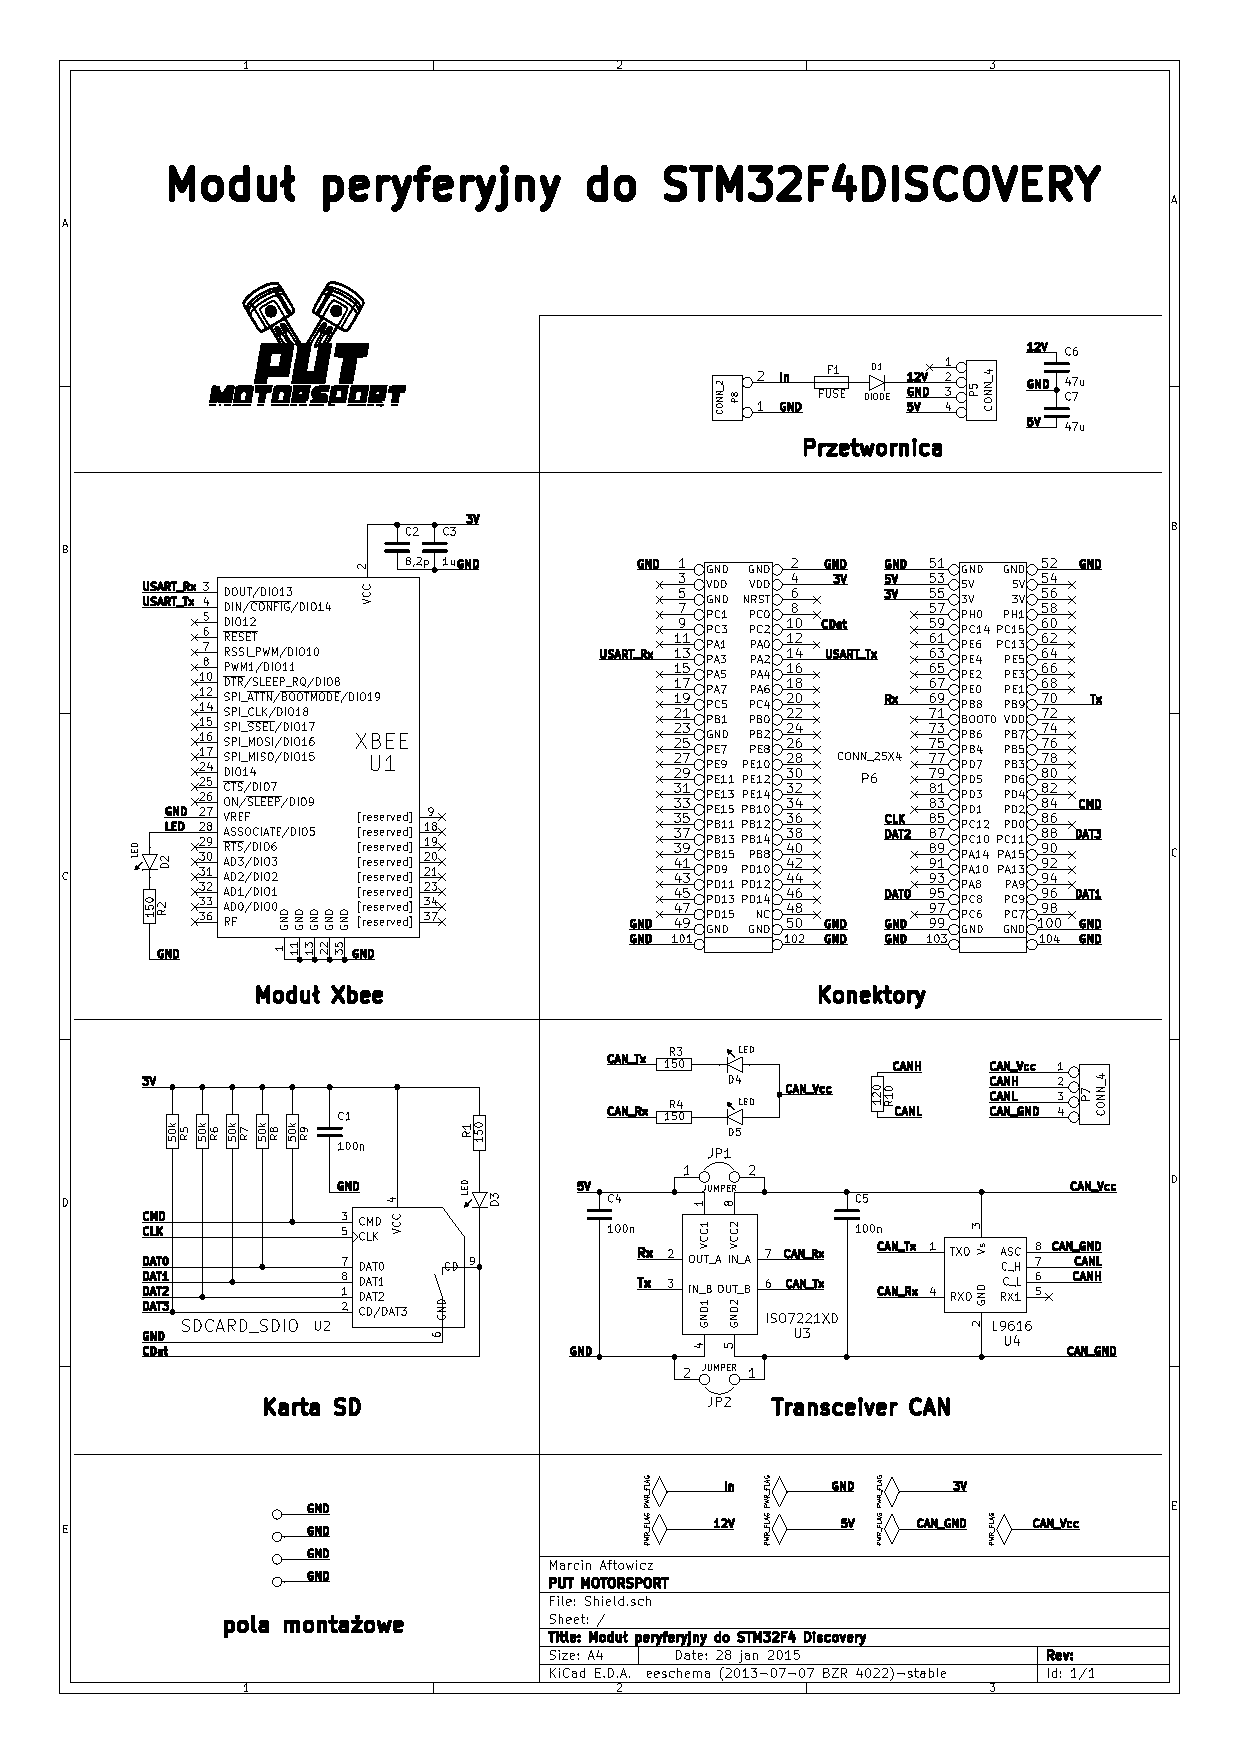
\includepdf[trim=0 0 -1cm 0, pages={1}]{figures/Motherboard_bw.pdf}
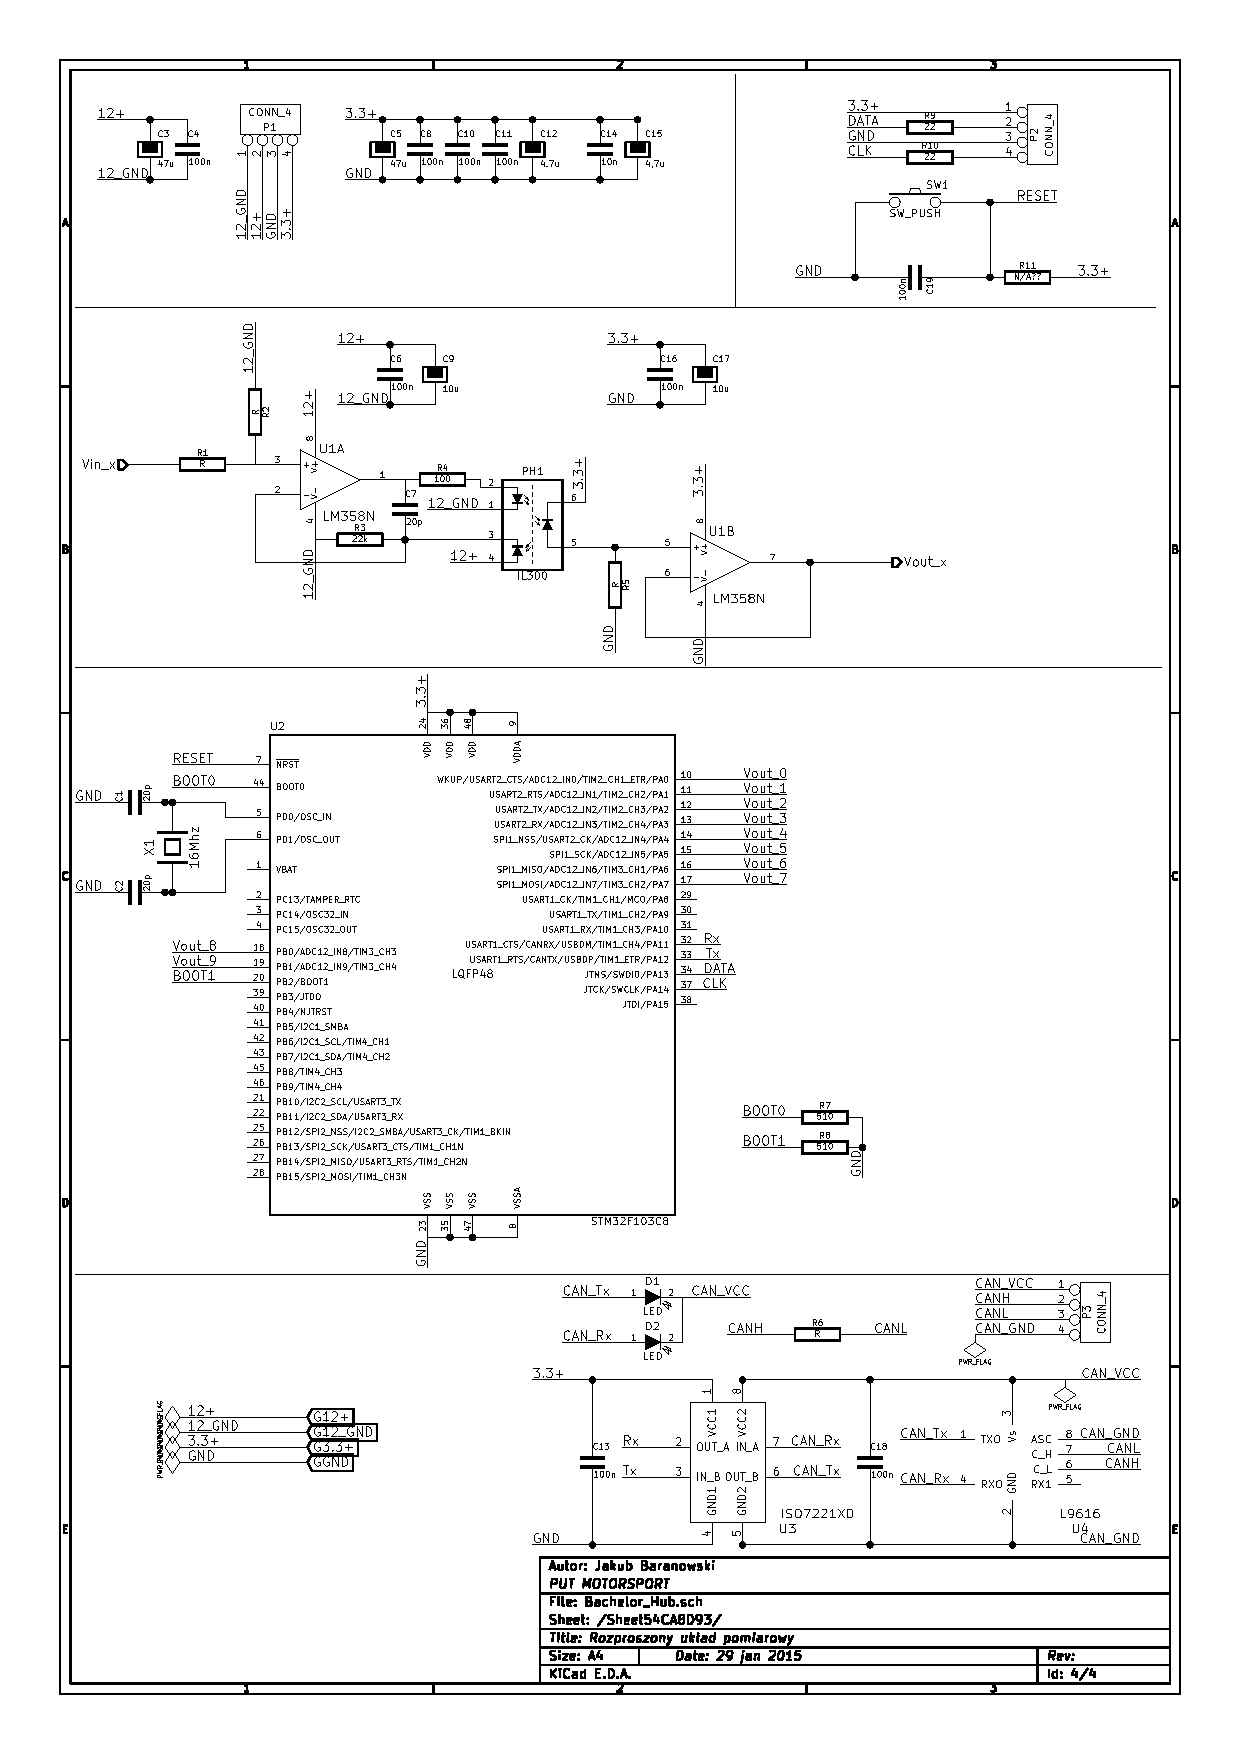
\includepdf[trim=-1cm 0 0 0, pages={1}]{figures/Bachelor_Hub.pdf}
\noindent



%%\input{plyta.tex}
%\cleardoublepage
\hypersetup{ linkcolor={black}}
\cleardoublepage

\bibliography{bibliografia}
\end{document}